\documentclass[conference]{IEEEtran}
\IEEEoverridecommandlockouts
% The preceding line is only needed to identify funding in the first footnote. If that is unneeded, please comment it out.
\usepackage{cite}
\usepackage{amsmath,amssymb,amsfonts}
\usepackage{algorithmic}
\usepackage{graphicx}
\usepackage{textcomp}
\usepackage{xcolor}
\def\BibTeX{{\rm B\kern-.05em{\sc i\kern-.025em b}\kern-.08em
    T\kern-.1667em\lower.7ex\hbox{E}\kern-.125emX}}

%\usepackage{amsmath,amssymb,amsfonts}
%\usepackage{algorithmic}
%\usepackage{graphicx}
%\usepackage{textcomp}
%\usepackage{xcolor}

%\usepackage{cite}
\usepackage{booktabs}   %% For formal tables:
                        %% http://ctan.org/pkg/booktabs
\usepackage{subcaption} %% For complex figures with subfigures/subcaptions
                        %% http://ctan.org/pkg/subcaption
\usepackage{array}
%\usepackage{amsmath,amsfonts}
%\usepackage{algorithm}
%\usepackage[noend]{algpseudocode}
%\usepackage{algorithmic}
%\usepackage{graphicx}
%\usepackage{textcomp}
\usepackage{float}
\usepackage{listings}
\usepackage{xspace}
\usepackage{multirow}
\usepackage{amsthm}
\usepackage{enumitem}

\newtheorem{definition}{Definition}
\usepackage{balance}
\usepackage{printlen}
\usepackage[skins]{tcolorbox}

%\usepackage{xcolor,pifont}
%\newcommand*\colourcheck[1]{%
%	\expandafter\newcommand\csname #1check\endcsname{\textcolor{#1}{\ding{52}}}%
%}
%\colourcheck{blue}
%\colourcheck{green}
%\colourcheck{red}

\newtcolorbox{myframe}[2][]{%
  enhanced,colback=white,colframe=black,coltitle=black,
  sharp corners,
  toprule=1.0pt,
  rightrule=0.3pt,
  leftrule=0pt,
  bottomrule=0pt,
  fonttitle=\itshape\scshape\large,
  left=0pt,right=5pt,top=5pt,bottom=3pt,
  attach boxed title to top right={yshift=-0.3\baselineskip-0.4pt,xshift=-5mm},
  boxed title style={tile,size=minimal,left=0.2mm,right=0.5mm,
    colback=white,before upper=\strut},
  title=#2,#1
}

%\newcommand{\code}[1]{{\footnotesize\textsf{#1}}}

\newcommand{\tool}{\textsc{DeepPDA}\xspace}

\newtheorem{Definition}{Definition}
\newtheorem{Claim}{Claim}
\newtheorem{Lemma}{Lemma}
\newtheorem{Theorem}{Theorem}

\newcolumntype{L}[1]{>{\raggedright\arraybackslash}p{#1}}
\newtheorem{observation}{Observation}
\newtheorem{property}{Property}
\newcommand{\code}[1]{{\footnotesize\texttt{#1}}}
\usepackage{amsthm}
 \definecolor{dkgreen}{rgb}{0,0.6,0}
\definecolor{gray}{rgb}{0.5,0.5,0.5}
\definecolor{mauve}{rgb}{0.58,0,0.82}
\lstset{frame=tb,
  language=Java,
  aboveskip=3mm,
  belowskip=3mm,
  showstringspaces=false,
  columns=flexible,
  basicstyle={\small\ttfamily},
  numbers=left,
  numberstyle=\tiny\color{gray},
  keywordstyle=\color{blue},
  commentstyle=\color{dkgreen},
  stringstyle=\color{mauve},
  breaklines=true,
  breakatwhitespace=true,
  tabsize=4
}


%\usepackage{tikz}
%\usetikzlibrary{shapes.arrows}
%\newcommand{\FancyUpArrow}{\begin{tikzpicture}[baseline=-0.3em]
%		\node[single arrow,draw,rotate=90,single arrow head extend=0.1em,inner
%		ysep=0.1em,transform shape,line width=0.03em,top color=green,bottom color=green!50!black] (X){};
%\end{tikzpicture}}

%\def\BibTeX{{\rm B\kern-.05em{\sc i\kern-.025em b}\kern-.08em
%    T\kern-.1667em\lower.7ex\hbox{E}\kern-.125emX}}


\begin{document}

%\title{A Fast and Accurate (Partial) Program Dependence Analysis Tool Using Neural Networks}
\title{Enabling Control-Flow and Dependence Analysis in (Partial) Programs Using Neural Networks}


\author{\IEEEauthorblockN{Aashish Yadavally}
\IEEEauthorblockA{%\textit{Computer Science Department} \\
\textit{University of Texas at Dallas}\\
Texas, USA \\
aashish.yadavally@utdallas.edu}
\and
\IEEEauthorblockN{Wenbo Wang}
\IEEEauthorblockA{\textit{Department of Informatics} \\
\textit{New Jersey Institute of Technology}\\
New Jersey, USA \\
ww6@njit.edu}
\and
\IEEEauthorblockN{Shaohua Wang}
\IEEEauthorblockA{\textit{Department of Informatics} \\
\textit{New Jersey Institute of Technology}\\
New Jersey, USA \\
davidshwang@ieee.org}
\and
\IEEEauthorblockN{Tien N. Nguyen}
\IEEEauthorblockA{\textit{Computer Science Department} \\
\textit{University of Texas at Dallas}\\
%City, Country \\
tien.n.nguyen@utdallas.edu}
%\IEEEauthorblockN{3\textsuperscript{rd} Given Name Surname}
%\IEEEauthorblockA{\textit{dept. name of organization (of Aff.)} \\
%\textit{name of organization (of Aff.)}\\
%City, Country \\
%email address or ORCID}
%\and
%\IEEEauthorblockN{4\textsuperscript{th} Given Name Surname}
%\IEEEauthorblockA{\textit{dept. name of organization (of Aff.)} \\
%\textit{name of organization (of Aff.)}\\
%City, Country \\
%email address or ORCID}
%\and
%\IEEEauthorblockN{5\textsuperscript{th} Given Name Surname}
%\IEEEauthorblockA{\textit{dept. name of organization (of Aff.)} \\
%\textit{name of organization (of Aff.)}\\
%City, Country \\
%email address or ORCID}
%\and
%\IEEEauthorblockN{6\textsuperscript{th} Given Name Surname}
%\IEEEauthorblockA{\textit{dept. name of organization (of Aff.)} \\
%\textit{name of organization (of Aff.)}\\
%City, Country \\
%email address or ORCID}
}

\maketitle

\begin{abstract}
%% Code fragments from developer forums often migrate to applications due
%% to the code reuse practice. Owing~to~the incomplete nature of such
%% code fragments, analyzing them to early determine the presence of
%% potential vulnerabilities is challenging. In this work, we introduce
%% \tool, a neural network-based program dependence analysis tool for
%% both complete and partial programs. Inspired from dependency parsing
%% in natural language processing, {\tool} models this as the
%% statement-pairwise dependence decoding, with the support of both
%% intra-statement context learning and inter-statement context learning.
%% Our empirical evaluation shows that \tool predicts the CFG and PDG
%% edges in complete Java and C/C++ code with the F-scores of {\bf
%%   94.29\%} and {\bf 92.46\%}, respectively. The F-scores for partial
%% Java and C/C++ code range from 94.29--97.17\% and from
%% 92.46\%--96.01\%, respectively. We test the usefulness of the PDGs
%% predicted by \tool (PDG\textsuperscript{*}) on the task of
%% method-level vulnerability detection (VD). We discover that the
%% performance of the VD tool utilizing PDG\textsuperscript{*} is only
%% 1.1\% less than that utilizing the PDGs generated by a program
%% analysis tool. Furthermore, we report that by leveraging the PDGs
%% predicted by DeepPDA, a machine learning-based VD tool can detect 14
%% real-world vulnerable code snippets from StackOverflow.
%% %for 99 vulnerable code snippets from
  %% %StackOverflow, a VD tool can correctly identify \_\_ of them.
  
Code fragments from developer forums often migrate to applications due
to the code reuse practice. Owing to the incomplete nature of such
code fragments, analyzing them to early determine the presence of
potential vulnerabilities is challenging. In this work, we introduce
\tool, a neural network-based tool to build program dependence graph
(PDG) for both complete and partial programs. We design {\tool} to
efficiently incorporate intra-statement and inter-statement contextual
features into statement representations, thereby modeling program
dependencies as a statement-pair dependence decoding task. Our
empirical evaluation shows that \tool predicts the CFG and PDG edges
in complete Java and C/C++ code with combined F-scores of 94.29\% and
92.46\%, respectively. The F-scores for partial Java and C/C++ code
range from 94.29\%--97.17\% and 92.46\%--96.01\%, respectively.

%We also test the usefulness of the PDGs predicted by \tool (PDG*) on
%the task of method-level vulnerability detection (VD). We discover
%that the performance of the VD tool utilizing PDG* is only 1.1\% less
%than that utilizing the PDGs generated by a program analysis
%tool. Furthermore, we report the detection of 14 real-world vulnerable
%code snippets from StackOverflow by a machine learning-based VD tool
%that employs the PDGs predicted by \tool for these code snippets.

\end{abstract}


%\begin{IEEEkeywords}
%component, formatting, style, styling, insert
%\end{IEEEkeywords}

\section{Introduction}

Integrating the utilization of program analysis (PA) tools early in the development process of modern, large-scale software systems is crucial in determining the weaknesses/vulnerabilities in the code. Consider, for instance, a scenario in which a developer wants to use an online question and answering (Q\&A) forum, e.g., StackOverflow (S/O), to learn how to use software libraries or frameworks. Typically, the answer to a posed question comes as a fragment/chunk of code, which later makes it to the production application, stemming from the copy-and-paste software reuse practice. Unfortunately, if the copied code fragment is vulnerable, i.e., possesses defects that one can potentially exploit, it will result in the application being prone to attacks. Verdi {\em et al.}~\cite{verdi-tse22} reviewed more than 72K C++ code snippets that migrated from 1,325 S/O answers, reporting a total of 99 vulnerable code snippets of 31 different types that made their way to 2,589 GitHub repositories.

Security researchers have proposed several automated approaches for vulnerability detection (VD) in software systems using program analysis (PA)~\cite{FlawFinder,RATS,viega2000its4,Checkmarx,HPFortify,Coverity}, as well as machine learning and deep learning (ML \& DL) \cite{fse21,chakraborty2020deep,zhou2019devign,li2018sysevr,li2018vuldeepecker} techniques. These approaches typically leverage program representations such as abstract syntax tree (AST), program dependence graph (PDG)~\cite{fse21,li2018vuldeepecker}, control-flow graph (CFG)~\cite{zhou2019devign}, data-flow graph (DFG)~\cite{zhou2019devign}, code property graph (CPG)~\cite{chakraborty2020deep}, etc., to model the vulnerable features. 
%However, extending such analyses to code snippets is not straightforward as they are often incomplete, unparseable, contain declaration/reference ambiguity, and may be interspersed between user comments. Currently, there exist tools such as PPA~\cite{ppa08}, which parse an incomplete code fragment to build the AST and extract data types in a best-effort manner, while StaType \cite{icse18} resolves the libraries and recovers only the fully-qualified names for references. However, the basic infrastructure for partial program analysis, i.e., for analyzing incomplete code is not yet available. 
%Such an infrastructure must include fundamental supports/services at the structural, semantic, and execution levels, thus enabling the static and dynamic analysis techniques to be built upon. 
%Let us refer to this as \textit{partial program analysis infrastructure}.
However, the PA tools employed to derive these program representations warrant the code to exist as complete program units, at the very least, at the method-level granularity. As a result, it is impossible to utilize such VD tools to find vulnerabilities in code snippets. A possible alternative would be to plug the code snippet into the method, resolve any ambiguities, and test it with a VD tool. However, such a strategy is limited. First, if a vulnerability is found, the efforts of integrating the code snippet into the existing method would be lost. Second, due to the black-box nature of DL models, we would not know the origin of the vulnerability, i.e., whether it arises due to the flawed code snippet or the existing part of the code.

Besides, analyzing code snippets is not straightforward as they are often incomplete, un-parseable, contain declaration/reference ambiguity, and are interspersed between user comments. Currently, there exist tools such as PPA~\cite{ppa08},~which parse an incomplete code fragment to build the AST and~ex\-tract data types in a best-effort manner, while StatType \cite{icse18} resolves the libraries and recovers only the fully-qualified names for references. However, deriving the program dependencies on incomplete code snippets is not yet possible. Let us call such an analysis, {\em partial program dependence analysis}.

In addition to vulnerability detection, such partial program dependence analysis is also beneficial to the other software engineering (SE) tasks that can tolerate a low level of errors and imprecision in building the dependencies. For example, consider code completion~\cite{codefill-icse22,facebook-icse21}, in which a model provides suggestions to complete partial code. Existing ML/DL-based code completion models are just based on the code sequences or utilize the syntactic structure in ASTs, but none leverage the program dependencies due to the nature of partial code. Next, consider the task of analyzing the code fragments in a bug report to connect it to the relevant source files for bug localization purposes~\cite{euler-fse19,icpc17}. Here too, a need for partial program dependence analysis can be observed.

In this work, we introduce \tool, a neural network-based tool to build
program dependence graph (PDG) for both complete and partial
programs. 

\begin{figure*}[hbt!]
\begin{center}
    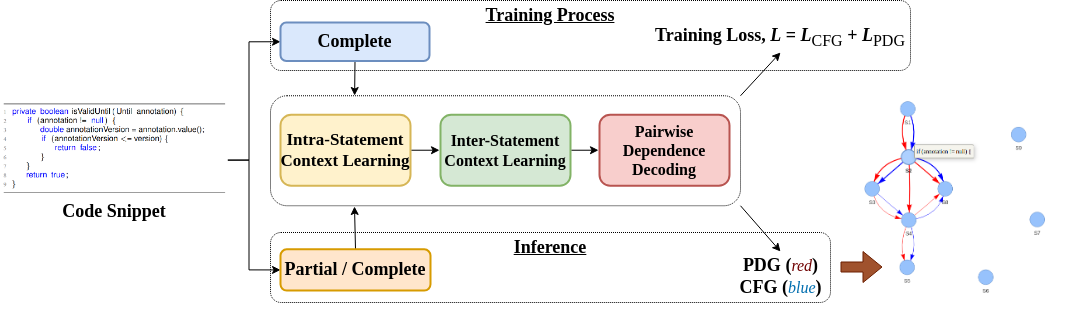
\includegraphics[width=\textwidth]{icse23-demo-figures/demo-arch3.png}
    \caption{\tool training and inference pipeline to enable dependence analysis for both partial and complete code.}
    \label{fig:model}
    \vspace{-10pt}
\end{center}
\end{figure*}

We draw motivation for such a data-driven, learning-based approach
from the following. First, ultra-large-scale software repositories,
e.g., GitHub (7M+ projects) and SourceForge (700k+ projects), contain
an enormous collection of programs. These repositories amount to 1B+
lines of code, 10M+ revision logs, and 3M+ issue reports. This wealth
of knowledge is an excellent source for {\tool}. Hindle {\em et
  al.}~\cite{naturalness-icse12} have shown that code has high
repetitiveness and predictability and can be captured well by
statistical models. Thus, we expect to build ML/DL models to learn
from those repositories.
%Second, Nguyen {\em et al.}~\cite{icse15} reported a high
%repetitiveness level for the sub-graphs in PDGs in open-source
%projects. Thus, {\tool} could learn the dependency structures
%extracted for whole programs in the existing code repositories and
%infer data types and program dependencies for partial programs. Third,
Second, in an empirical study on the repetitiveness, containment, and
composability of PDGs in open-source projects, Nguyen {\em et
  al.}~\cite{msr16} reported that among 17.5M PDGs with 1.6B PDG
subgraphs, 14.3\% of the PDGs have all of their subgraphs repeated
across different projects. Furthermore, in 15.6\% of the PDGs, at
least 90\% of their subgraphs are likely to have appeared before in
other projects.
%Second, Nguyen {\em et al.}~\cite{icse15} reported a high
%repetitiveness level for AST code structure in open-source
%projects. Thus, {\tool} infrastructure could help learn
%structure-level information from the ASTs extracted for whole programs
%in the existing code repositories and infer data types, partial ASTs
%for partial programs. Third, in an empirical study on the
%repetitiveness, containment, and composability of PDGs in open-source
%projects, the PI group~\cite{msr16} reported that among 17.5M PDGs
%with 1.6B PDG subgraphs, 14.3\% of the PDGs have all of their
%subgraphs repeated across different projects. Furthermore, in 15.6\%
%of the PDGs, at least 90\% of their subgraphs are likely to have
%appeared before in other projects.
%Thus, {\tool} could learn from PDGs with complete program dependencies retrieved from existing code repositories and derive the dependencies for the (partial) code fragment under study. The PI group also reported a high repetitiveness level for AST code structure in open-source projects~\cite{icse15}.
Thus, {\tool} could learn semantic-level information from the PDGs
with complete program dependencies retrieved from existing code
repositories and infer such dependencies for the partial code.


We design {\tool} to efficiently incorporate intra-statement and
inter-statement contextual features into statement representations,
thereby modeling program dependencies as a statement-pair dependence
decoding task. The key philosophy that drives our work is that the
dependency analyses of partial code can be learned from the analysis
of entire programs in the wealth of information obtained from
ultra-large-scale, open-source software repositories.


%Our key contributions are as follows:
%\begin{enumerate}
%    \item enable construction of interactive control-flow and program dependence graphs for \underline{partial} code snippets.
%    \item provide support to both Java and C++.
%    \item observe $\sim380\times$ markup against Joern PA tool.
%\end{enumerate}

\section{Our Approach}
\label{sec:approach}

Neural network-based dependency parsing approaches in natural language processing (NLP)~\cite{chen-manning-2014-fast} project words in a sentence into an embedding space to successfully learn the semantic relationships between them. Thus, we sought motivation for \tool's design, geared towards learning the control-flow and program dependencies between statements in programs. Moreover, the quality of the statement embeddings determines how accurately our tool can predict the program dependence relations. Thus, enhancing them by incorporating context from both within and across the statements is crucial. For example, the knowledge of the declaration of a variable in one statement and its reference in another helps identify the \textit{def-use} chain between them. Also, it is important to model the effect that a statement has on the other statements. For example, such information helps identify the scope of a given statement. Finally, we model our problem as a pairwise dependence decoding task, wherein the combination of all predicted edges across the statement pairs in a program can be formalized as a directed graph, i.e., its CFG/PDG.

\subsection{Model Architecture}
\label{sec:arch}

In Figure~\ref{fig:model}, we present the general model architecture of \tool. We incorporate various context-learning modules to capture the well-defined structure and semantics in source code. In this section, we describe each of these components.

\subsubsection{Contextualization}
Effective contextualization is a key idea driving \tool's design. We enable this via a hierarchical, self-attention network (SAN)-based architecture, where each sub-network is intended to capture different aspects of contextualization. Its details are as follows:

\begin{itemize}[leftmargin=*, listparindent=\parindent, parsep=0pt, itemsep=\topsep]
%\begin{itemize}[listparindent=\parindent, parsep=0pt, itemsep=\topsep]
    \item \underline{\textit{Intra-Statement Context Learning (IntraS-CL)}}. To relay the syntactic and semantic knowledge of code tokens within individual statements globally, intra-statement contextualization is crucial. We enable this via a \textit{1-Layer} (i.e., $N_X$$=$$1$) Self Attention Network (1L-SAN). The self-attention layer in an 1L-SAN inputs $x_1, x_2, ..., x_n \in \mathbb{R}^d$, performs self-attention once by projecting the inputs from all attention heads $\in\mathbb{R}^{d_h}$ into the head dimension space $d_h$ via linear transformations, and generate outputs $y_1, y_2, ..., y_n \in\mathbb{R}^d$ which are linear combinations of the concatenated attention head values. We use one attention head (i.e., $h$$=$$1$) for the self-attention layer in 1L-SAN, and the size of the input representations, i.e., $d$ is set to 512.

    \hangindent=0.7cm For a program comprising $N$ statements $s_1, s_2, ..., s_N$, \tool takes as input a concatenation of $N$ sequences of $M$ tokens each, $\langle t_1^{(1)}$, $t_2^{(1)}$.., $t_M^{(1)} \rangle$, ..., $\langle t_1^{(N)}$, $t_2^{(N)}$.., $t_M^{(N)} \rangle$. Next, each token sequence $\langle t_1^{(i)}$, $t_2^{(i)}$.., $t_M^{(i)} \rangle$ is input to the 1L-SAN for intra-statement contextualization. Previous works~\cite{radford2019language, liu2019roberta} have demonstrated the advantages of a byte-level Byte-Pair Encoding (BPE)-scheme for tokenization. We follow suit to train a byte-level BPE tokenizer for converting a given statement into a sequence of tokens. Here, $M$ is the maximum number of tokens allowed in a statement. For statements with token sequences having ${<}M$ tokens, a special \textit{[PAD]} token is appended. In contrast, token sequences having ${>}M$ tokens are truncated to $M$ tokens.

    \item \underline{\textit{Inter-Statement Context Learning (InterS-CL)}}. The knowledge of the surrounding statements in the context of a given statement helps \tool model the dependencies between them better. We enable this via a multi-layer bidirectional Transformer encoder based on Vaswani {\em et al.}~\cite{Vaswani-2017}. Owing to its common usage, we will omit the details on Transformers' model architecture and will refer the readers to ~\cite{Vaswani-2017}. We set the number of layers in the Transformer encoder, i.e., $N_Y$ to 6. 
    We employ 4 attention heads
    %, i.e., $h$$=$$4$ 
    to increase parallelization 
    %(since $d_h$$=$$\frac{d}{h}$, i.e., $d_h$$=$$128$) 
    and learn different aspects of the syntactic and semantic structure in the statements, while still being interpretable. We also set the feed-forward module size to be 4 times that of the size of the input representations $d$, i.e., 2048. Overall, Transformer in InterS-CL phase inputs local context-aware statement representations $u_i \in \mathbb{R}^d$ for all statements $s_i$ in a given program, and outputs statement representations $v_i \in \mathbb{R}^d$ that are both local and global context-aware.
\end{itemize}

\subsubsection{Pairwise Dependence Decoding}
From the sequence of contextualized statement representations $v_i \in\mathbb{R}^d$ corresponding to all the statements $s_i$ in a program, pairs such as $\langle v_x, v_y \rangle$ (1$\leq x, y\leq$ N) are taken to detect the presence of CFG/PDG edges between two statements $s_x$ and $s_y$. We leverage 2-layered multi-layer perceptron networks (each for detecting the CFG and PDG edges, i.e., MLP\textsubscript{CFG} and MLP\textsubscript{PDG}, respectively) in this phase, which are scored as per the following equation:
\begin{equation}
\centering
    score\textsubscript{rel}(x, y) = MLP\textsubscript{rel}(v_x \circ v_y \circ (v_x * v_y) \circ |v_x - v_y|) \nonumber
\end{equation}
where $\circ$, $*$ and $|.|$ correspond to concatenation, element-wise
product, and absolute element-wise difference operations respectively;
and \textit{rel} represents either the control-flow or program
dependence relations. 
%and \textit{rel} $\in$ \{CFG, PDG\}. 
Attaining a $score\textsubscript{rel}(x, y) >
0.5$ represents the detection of the corresponding CFG/PDG edge from
statement $s_x$ to statement $s_y$. The combination of all the CFG/PDG
edges extracted via such an arc-factored approach is realized as the
CFG/PDG for the given program.

\subsection{\bf Training Process}
Training \tool requires the knowledge of whether a CFG or PDG edge occurs between any two statements in the program. This is due to its design as an inter-statement dependence prediction problem. Leveraging PA tools to extract such ground-truth information, however, requires the program to be complete, parseable, and at a minimum, at the method level. Following this, the training objective loss (i.e., $\mathcal{L}$) for our model can be computed as ${\mathcal{L} = \mathcal{L}\textsubscript{CFG} + \mathcal{L}\textsubscript{PDG}}$,
%\begin{equation}
%    \centering
%    $$\mathcal{L} = \mathcal{L}\textsubscript{CFG} + \mathcal{L}\textsubscript{PDG}$$
%\end{equation}
where $\mathcal{L}\textsubscript{CFG}$ and $\mathcal{L}\textsubscript{PDG}$ are losses for CFG and PDG edge-decoding, respectively, each computed as the sums of all binary-cross entropy (BCE) losses corresponding to the CFG and PDG edge predictions for all statement pairs in the program.
%Note that the inter-statement losses corresponding to the edges from/to the zero-padded statements do not contribute to either $\mathcal{L}\textsubscript{CFG}$ or $\mathcal{L}\textsubscript{PDG}$. The model parameters which are learned to minimize $\mathcal{L}$ include learnable embeddings (token, token position, statement type, and statement position), attention, Tr-FFNN (i.e., feed-forward neural network in Transformer encoder), MLP\textsubscript{CFG}, and MLP\textsubscript{PDG}.

%Overall, \tool has about 39M parameters.

\subsection{\bf Inference for Dependency Discovery}
\label{sec:inference}
Despite being trained on only complete code, one can leverage \tool to extract the control-flow and program dependence edges for both complete and partial code. Let us assume that the maximum number of statements allowed in our model is $N$. Leveraging it to infer dependencies for programs with ${\leq}N$ statements is straightforward, as in these cases, each statement is simply contextualized over all the other statements in the program. However, for programs with ${>}N$ statements,
%, we have the following strategies: (a) train a model with a higher value of $N$, (b) 
we 
chunk the program into $N$-statement code fragments, predict CFG/PDG edges for each of the code fragments independently, and finally, combine the CFG/PDG predictions for all the fragments. For example, if a trained model allows a maximum of 16 statements, to predict for a program with 46 statements, we break it down into code fragments with 16, 16, and 14 statements, respectively.

\section{Preliminary Evaluation}

\subsection{Methodology}

\subsection{Results}

\begin{table}[H]
  \centering
  \small
  \caption{Effectiveness Evaluation on Complete Methods from Java and C++ Programming Languages}
\begin{tabular}{c|c|c|c|c}
\hline
\textbf{P/L}         & \textbf{Graph}   & \textbf{Precision} & \textbf{Recall} & \textbf{F-Score} \\ \hline
Java                 & \textit{CFG}     & 98.31              & 98.58           & 98.44            \\
                     & \textit{PDG}     & 89.89              & 87.53           & 88.70            \\
                     & \textit{Overall} & 94.75            & 93.83           & \textbf{94.29}   \\
\hline
\multirow{3}{*}{C++} & \textit{CFG}     & 96.86            & 96.92         & 96.89           \\
                     & \textit{PDG}     & 86.00            & 88.69         & 87.33           \\
                     & \textit{Overall} & 91.10            & 93.87         & \textbf{92.46}  \\
\hline
\end{tabular}
\label{tab:intrinsic-java}
\end{table}
%% Should originally belong to \subsection{Working Demo}.
%% Moving it here to move the image up a page.
\begin{figure*}[hbt!]
\centering
%%%%%%%%%%%%%%%%%%%%%%%%%%%%%%%%%%%%%
\begin{subfigure}[b]{.4\textwidth}
\begin{lstlisting}[basicstyle=\scriptsize\sffamily, stepnumber=1, numbers=left, numbersep=-6pt, framexleftmargin=0mm, framexrightmargin=0mm, language=Java, emph={allGames}]
    List<Game> allGames = gameMapper.getAllGamesByLeague(league);
    for (Game game : allGames) {
        game.getTeam1().setGame(game);
        game.getTeam2().setGame(game);
    }
    Collections.sort(allGames, new GameComparator());
\end{lstlisting}
%\caption{A listing}
\end{subfigure}
%%%%%%%%%%%%%%%%%%%%%%%%%%%%%%%%%%%%%%%%%%%%
\begin{subfigure}[b]{.4\textwidth}
\begin{lstlisting}[basicstyle=\scriptsize\sffamily, stepnumber=1, numbers=left, numbersep=-6pt, framexleftmargin=0mm, framexrightmargin=0mm, language=java, emph={annotationVersion}]
    private boolean isValidUntil(Until annotation) {
        if (annotation != null) {
            double annotationVersion = annotation.value();
            if (annotationVersion <= version) {
                return false;
            }
        }
        return true;
    }
\end{lstlisting}
\end{subfigure}
%%%%%%%%%%%%%%%%%%%%%%%%%%%%%%%%%%%%%%%%%%%%
\begin{subfigure}[b]{.45\textwidth}
  \centering
  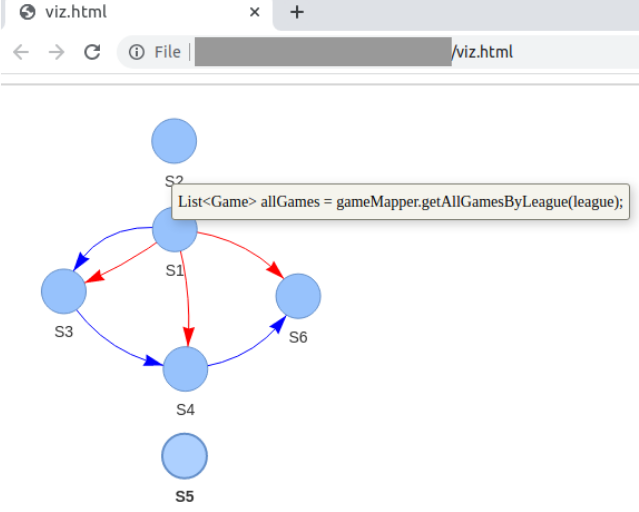
\includegraphics[width=0.7\linewidth]{icse23-demo-figures/lst-partial2.png}
  \vspace{0.75cm}
\end{subfigure}
%%%%%%%%%%%%%%%%%%%%%%%%%%%%%%%%%%%%%%%%%%%%
\begin{subfigure}[b]{.45\textwidth}
  \centering
  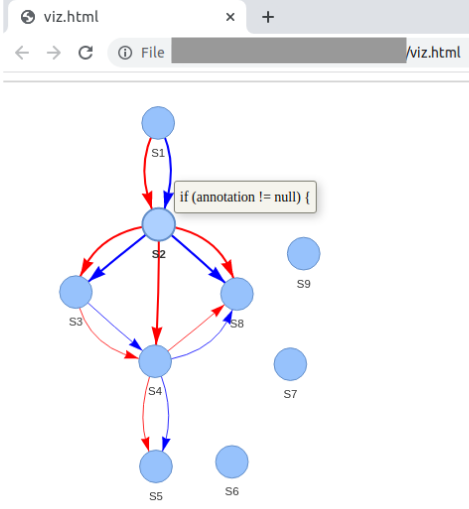
\includegraphics[width=0.7\linewidth]{icse23-demo-figures/lst-complete2.png}
\end{subfigure}
%%%%%%%%%%%%%%%%%%%%%%%%%%%%%%%%%%%%%%%%%%%%
\caption{Partial (top-left) and complete (top-right) Java code listings and their CFG/PDGs output by \tool (bottom).}
\label{fig:demo}
\end{figure*}

\section{Getting Started with \tool}
\subsection{Environment Setup}
\tool was implemented as a Python package using 
several libraries including \code{pytorch}, \code{transformers}, \code{pyvis},
etc. A working environment can be set up with the help of 
\code{conda} package manager in the Anaconda Python distribution~\cite{anaconda}, 
and the provided YAML configuration file with the following 
command: \code{\$ conda env create -f environment.yml}

\subsection{Usage}
The prototype for \tool can be run in the virtual environment as a command-line utility as follows:

\noindent \code{\$ python infer.py -i <input-path> -o <output-format>}
\begin{itemize}
    \item \code{-i}: Path to a \code{.txt} file containing the code snippet, or a directory containing multiple input \code{.txt} files. 
    \item \code{-o \{json|html\}}: \code{json} option outputs a JSON file containing predicted CFG/PDG edge information between the statements in the code snippet(s). \code{html} option draws an interactive directed graph bearing CFG (\textit{blue}) and PDG (\textit{red}) edges, further saving it as an HTML file(s). 
\end{itemize}

After loading the pre-trained dependency inference model, \tool takes a blazing quick 
%\textcolor{red}{0.\_\_} seconds on an Intel 8\textsuperscript{th} generation CPU and is even faster on a machine with a GPU ($\sim$0.02 seconds with an Nvidia Quadro P4000 GPU).
$\sim$0.02 seconds on a machine with an Nvidia Quadro P4000 GPU.

\subsection{Working Demo}
In Figure~\ref{fig:demo}, we illustrate a working demonstration of \tool. At the top, we present two Java code snippets: partial (left), and complete (right). The corresponding CFG/PDGs output by \tool are drawn at the bottom. The control-flow edges and program dependence edges are highlighted in \textit{blue} and \textit{red} colors respectively. Clicking on a node bolds all edges coming to, or leaving the node. In addition, hovering over a node lists the corresponding statement in a text box.

In the partial code snippet (left), statement-block $S_3$--$S_4$ iterates over the variable \code{allGames} defined in statement $S_1$. Due to the loop dependence, program (data)-dependence edges $S_1{\rightarrow}S_3$ and $S_1{\rightarrow}S_4$ are identified (left-bottom). Besides, a \textit{def-use} chain and consequently, a data-dependence edge $S_1{\rightarrow}S_6$  over the identifier \code{allGames} is also identified.

For the complete code snippet (right), all control-flow edges are predicted accurately. In addition, \tool predicts all but one control-dependence edge, that from $S_2{\rightarrow}S_7$. However, given that it correctly identifies the control-flow edge between $S_2$ and $S_7$, it is likely that it was not able to conclude whether $S_2$ determines the execution of $S_7$, resulting in the miss.

Statements such as "\code{\{}" or "\code{\}}" are not syntactic statements, and do not share a dependence relation with other statements in the code snippet. Thus, our tool draws them as free nodes $S_5$ (left-bottom); $S_6$, $S_7$, and $S_9$ (right-bottom) in the graphs.

\subsection{Tool Availability}
All code and data used to build and run \tool is available at {https://github.com/deeppda-icse23/DeepPDA}. Also, our video demo can be found at \textcolor{red}{{Add.Youtube.video.link}}.
\section{Related Work}
%\subsection{Dependency Parsing \& Link Prediction}
%We seek inspiration for our problem setting from Chen and Manning~\cite{chen-manning-2014-fast}, who first proposed a neural network-based approach to dependency parsing. The major benefits we envision to such a formulation include a significant speedup in dependency discovery and the extendibility of program dependence analysis to partial programs. However, employing a transition-based parsing technique~\cite{chen-manning-2014-fast} requires excessive feature engineering, while also assuming the projectivity of the dependency tree. This limits the applicability of such approaches to source code. In contrast, neural graph-based dependency parsing appoaches'~\cite{kiperwasser-goldberg-2016-simple, DBLP:conf/iclr/DozatM17} outputs can be non-projective. However, unlike with graph-based dependency parsing, our output is not just one of the possible valid trees (or the maximum spanning tree). Rather, program dependence graphs are directed and cyclic structures. Thus, we plan to design the dependence decoding stage by extending the link prediction~\cite{10.5555/3327345.3327423} task to all possible statement pairs, the combination of all of which can be formalized as the predicted CFG/PDG.

%\subsection{Probabilistic Graphical Models}
We seek inspiration for our problem setting from Chen and Manning~\cite{chen-manning-2014-fast}, who first proposed a neural network-based approach to dependency parsing. The major benefits we envision to such a formulation include a significant speedup in dependency discovery and the extendibility of program dependence analysis to partial programs. 
%In SE domain, 
Specific to the SE domain, 
%the proposed research 
this research
is loosely related to works that leverage probabilistic models to enhance the program dependence graph (PDG). Probabilistic PDG~\cite{baah-issta08-probabilistic} is an augmentation of the structural dependencies represented by a PDG with estimates of statistical dependencies between node states derived from test cases. Feng et al.~\cite{feng-paste10} propose Error-Flow Graph as a Bayesian Network, constructed from the dynamic dependence graphs of the runs. Bayesian Network-based Program Dependence Graph (BNPDG)~\cite{yu-jss17-bayesian} is capable of inferring the dependencies across non-adjacent nodes. MOAD (Modeling Observation-based Approximate Dependency)~\cite{lee-scam19-moad} reformulates program dependency as the likelihood that one program element is dependent on another, instead of a boolean relationship.  Lee~\cite{lee-icse20} proposes a scalable approximate program dependence analysis by estimating the likelihood of dependence. It uses lexical analysis~\cite{lee-jss20}, partial observations on executions, and the merging of static and observation-based approaches. Those approaches leverage the knowledge from the executions to enhance the PDG for complete code. In contrast, we aim to use neural networks for deriving dependencies for both partial and complete code.

\section{Conclusion and Future Work}
We introduce a neural network-based program dependence analysis tool, \tool, which extends the construction of CFG/PDGs to partial code snippets. Owing to the significant speed markup ($\sim$380$\times$), we envision an opportunity for the integration of such a tool in the software development process, which will help facilitate real-time program analysis. Our tool can also benefit SE tasks such as vulnerability detection (VD), code completion, fault localization, etc., that can tolerate low levels of inaccuracies. The current prototype is highly accurate and supports Java and C/C++ at this point -- we plan to conquer other programming languages as well. In the future, we seek to combine our tool with existing PA tools, while also exploring cross-segment dependency-capturing strategies, so as to make it robust across larger codebases. 


%\input{intro1}
%\input{motiv1}
%\input{overview}
%\input{our_approach}
%\input{empirical_eval}
%\input{results-effectiveness}
%\input{miss.tex}
%\input{results_rq2}
%\input{results_rq3}
%\input{discussion}
%\input{related_work}
%\section{Conclusion and Future Work}
We introduce a neural network-based program dependence analysis tool, \tool, which extends the construction of CFG/PDGs to partial code snippets. Owing to the significant speed markup ($\sim$380$\times$), we envision an opportunity for the integration of such a tool in the software development process, which will help facilitate real-time program analysis. Our tool can also benefit SE tasks such as vulnerability detection (VD), code completion, fault localization, etc., that can tolerate low levels of inaccuracies. The current prototype is highly accurate and supports Java and C/C++ at this point -- we plan to conquer other programming languages as well. In the future, we seek to combine our tool with existing PA tools, while also exploring cross-segment dependency-capturing strategies, so as to make it robust across larger codebases. 


\balance
\bibliographystyle{IEEEtran}

\bibliography{reference,icse21IntVD,FL}



\end{document}
